\chapter{Metodologia}

Em \cite{winikoff2014testability} um grafo de controle de fluxo foi utilizado para avaliar a testabilidade de um sistema BDI. A proposta deste trabalho é avaliar a testabilidade de um SMA utilizando o $\mathcal{M}$oise$^{+}$ como modelo de organização e empregando RP como ferramenta de descrição e análise.  

foi transformado em uma RP Figura \ref{fig:cf_rp} seguindo a seguinte metodologia.



Partindo como base o trabalho de \cite{winikoff2017bdi} o grafo de controle de fluxo apresentado na Figura \ref{fig:control_fluxo} será utilizado para apresentar a metodologia de transformação de controle de fluxo para RP. Na conversão de controle de fluxo para RP é considerado que cada nó será transformado em um lugar, e as ligações entre os nós, as arestas, são convertidas em transições que são conectados aos lugares por arcos. Logo o nó \textbf{S} que é o início do controle de fluxo é transformado no lugar \textbf{S}. Os lugares \textbf{S} e \textbf{A1} são conectados por dois arcos e pela transição \textbf{t0}, que é a transição disparada ao começar o programa.

O nó \textbf{a1}, está ligado a outros dois nós em uma estrutura de divisão de caminhos, onde uma das arestas significa a falha e liga com o nó \textbf{a2} e outra quando a ação tem sucesso acessando o nó \textit{Y} que representa que o programa foi realizado com sucesso. Para a transformação na RP é necessário incluir a transição \textbf{t1}, que é disparada quando a ação \textbf{a1} falha, unindo o lugar \textbf{A1} a \textbf{A2}, e também a transição \textbf{t6} unindo o lugar \textbf{A1} ao lugar \textbf{Y}, transição que é disparada quando a ação \textbf{a1}  é bem sucedida. Esta primeira etapa é apresentada na Figura \ref{fig:4-fluxo-rp0.png}.

\begin{figure}[ht]
    \centering
    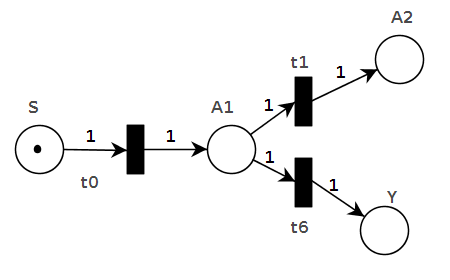
\includegraphics[scale=0.4]{imagens/4-fluxo-rp0.png}
    \caption{RP inicial.}
    \label{fig:4-fluxo-rp0.png}
\end{figure}

Como pode ser visto na Figura \ref{fig:cf_rp} a dinâmica da RP inicia pela indicação da \textit{ficha} no lugar \textbf{S}, quando a transição \textbf{t0} é disparada a ficha é movida para o lugar \textbf{A1}. Os arcos possuem o valor 1, significando que uma ficha já tem a capacidade de disparar aquela transição.

Em \textbf{A1} há uma estrutura de divisão entre diferentes sequências, onde e a transição \textbf{t6} é disparada quando é possível realizar a ação, indo assim para um lugar \textbf{Y} que corresponde à execução bem sucedida do programa, e finalmente para \textbf{E} que é o encerramento do programa. A transição \textbf{t1} é acionada quando o agente não consegue executar a ação \textbf{a1}, direcionando assim para o \textbf{A2}, esta ação pode ser bem sucedida, indo para a transição \textbf{t7}, ou falhar e ir para a transição \textbf{t2}, operando semelhante ao apresentado no \textit{lugar} \textbf{A1}.

%Como pode ser visto na Figura a dinâmica da RP inicia pela indicação da \textit{ficha} no lugar \textbf{S}, quando a transição \textbf{t0} é disparada a ficha é movida para o lugar \textbf{A1}. Neste lugar tem uma escolha entre diferentes sequências, onde e a transição \textbf{t6} é disparada quando é possível realizar a ação, indo assim para um lugar auxiliar \textbf{aux\_A1}, sendo assim possível disparar a transição \textbf{t10} que leva até ao lugar \textbf{Y} que corresponde à execução bem sucedida do programa, e finalmente para \textbf{E} que é o encerramento do programa. A transição \textbf{t1} é acionada quando o agente não consegue executar a ação, direcionando assim para o \textit{A2}, esta ação pode ser bem sucedida, indo para a transição \textbf{t7}, ou falhar e ir para a transição \textbf{t2}, operando semelhante ao apresentado no \textit{lugar} \textbf{A1}.

\begin{figure}[ht]
    \centering
    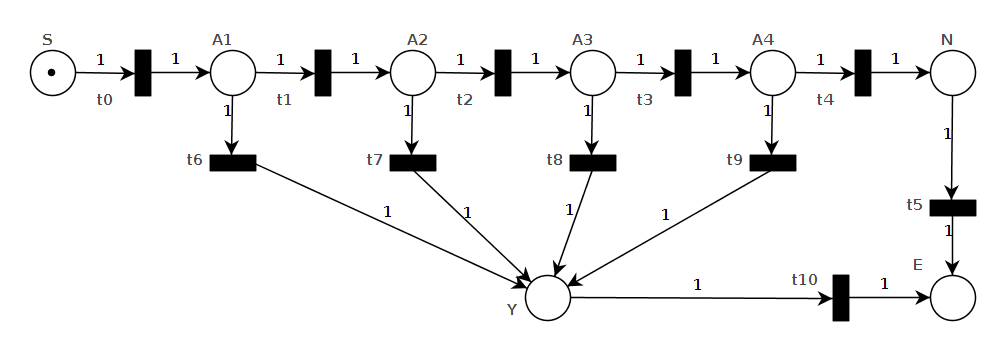
\includegraphics[scale=0.4]{imagens/4-fluxo-rp2.png}
    \caption{RP do grafo de controle de fluxo.}
    \label{fig:cf_rp}
\end{figure}

No método de \cite{winikoff2014testability,winikoff2017bdi} a avaliação de testabilidade é baseada na árvore de planos-metas, onde os objetivo tem como filhos os plano que são aplicáveis a ele, e cada instância do plano tem como filhos os sub-objetivos que ele publica, mas ainda apenas no nível de metas e ações. No contexto deste trabalho é necessário avaliar em múltiplos níveis que não estavam previsto em outros trabalhos, como missões, papéis e metas.

Em \cite{winikoff2014testability} a árvore de planos-metas é o pilar para seu trabalho, neste a avaliação da testabilidade no $\mathcal{M}$oise$^{+}$ será baseada no esquema social da especificação social, que é uma árvore de decomposição de metas. Para realizar a conversão do esquema social para RP é necessário convencionar a relação dos o operadores apresentados na legenda da Figura \ref{fig:es_exemplo} e sua RP equivalente.

\begin{itemize}

\item Operador \textit{sequência}: representa uma cadeia de metas em sequência. A meta \textbf{G10} inicia a sequência, caso a transição \textbf{t1} for iniciada a ficha é retirada de G10 e é colocada em \textbf{G13}, permitindo assim o seguimento da cadeia. 

\item Operador \textit{escolha}: apenas uma das metas, \textbf{G8} ou \textbf{G9} podem ser adotadas, para isso o lugar \textbf{G7} recebe uma restrição, quando uma transição for disparada e a ficha for inserida no lugar \textbf{G7}, a outra transição será desabilitada, não permitindo assim que a outra meta seja realizada. 

\item Operador \textit{paralelismo}: significa que as metas \textbf{G5} e \textbf{G6} podem progredir paralelamente e de modo assíncrono, mas a transição \textbf{t1} só será disparada quando as duas metas estiverem concluídas.

\end{itemize}

\begin{figure}[ht]
\centering
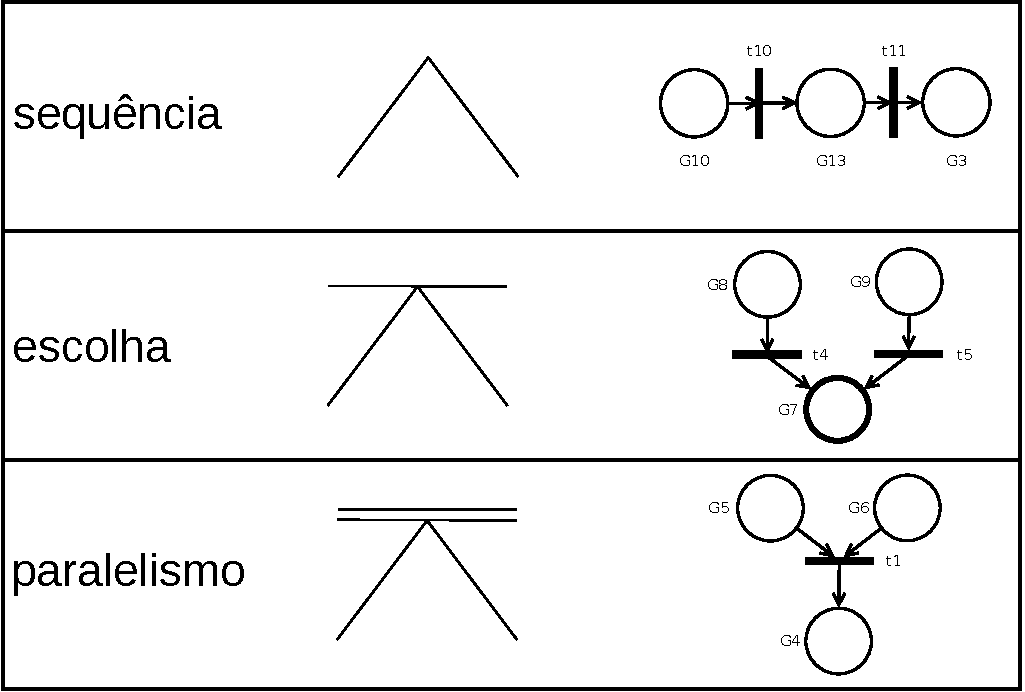
\includegraphics[scale=0.4]{imagens/4-relacao-moise-rp.pdf}
\caption{Relações dos operadores para Rede de Petri.}
\label{fig:moise_rp}
\end{figure}

Com a relação para a transformação dos operadores do esquema social para RP é possível criar a estrutura básica da rede, onde agora cada meta será um \textit{lugar}, semelhante ao que foi realizado na Figura \ref{fig:4estrutura_basica} onde cada ação foi transformado em um \textit{lugar}.  

Para atender ao nível organizacional é necessário utilizar recursos que não são disponíveis nas RP ordinárias, os recursos necessários são encontrados nas RP coloridas. As fichas coloridas são etiquetas que representam os papéis da organização, os lugares se associam ao conjunto de cores das fichas, ou seja, sendo os lugares metas, então cada lugar terá a cor associada ao conjunto de papéis relacionados e de acordo com a especificação deôntica é possível correlacionar com a missão que representa aquele lugar.

LIVRO RP pág 90 Associação de funçoes aos arcos, falar sobre os papéis e o valor das transições.

%Iniciando pela árvore de metas globais da Figura \ref{fig:es_exemplo}, e utilizando os operadores da Figura \ref{fig:moise_rp} a árvore é transformada em RP para cada missão, ainda de maneira isolada Figura \ref{fig:missoes_rp}. O processo começa lendo a árvore da esquerda para a direita da parte inferior, e transformando as metas em lugares da RP, utilizando os operadores relacionados, até que um conjuntos de meta para finalizar a missão seja concluída.